\section{Interaction Engineering - Fragenkatalog}
\subsection{Introduction}
\begin{enumerate}
	\item Erkläre Stärken und Schwächen des Menschens und des Computers in der Human-Computer Interaction!
	\begin{table}[!h]
		\centering
		\begin{tabular}{|p{20em}|p{20em}|}
			\hline
			Mensch & Computer\\
			\hline
			\tabitem Kreativität & \tabitem 'exakte'\footnote{Denke an max. Genauigkeit von Fließkommazahlen!} Berechnungen\\
			\tabitem Abstrahieren und Erzeugen von Modellen & \tabitem stundenlanges Ausführen derselben Aufgabe ohne zu Ermüden\\
			\tabitem auf Unerwartetes reagieren& \tabitem exakter Speicher (Gedächtnis)\\
			\hline
		\end{tabular}
		\caption{Stärken des Menschen und Computers in HCI. (Särken = Schwächen des anderen!)}
		\label{strength_of_hc}
	\end{table}
	
	\item Kernunterschied bei der Entwicklung von computional solutions und interactive solutions
	\begin{itemize}
		\item Interaction: Kernfaktor ist das Human Computer Interface
		\item Computational: Kern ist effizienter Algorithmus(?)
		\item Rechenleistung steigt immer weiter während menschliche Aufnahmefähigkeit stagniert/konstant ist
		\item Kernfaktor bei der Informationsverarbeitung durch den Menschen ist das Interface
		\item $\Rightarrow$ Interaction soll smooth und effizient; Feedback soll reich an Informationen und instantan sein
		\item HC-Interaction - Mensch und Computer gehen Hand in Hand, jeder erfüllt die Aufgaben, die er am besten lösen kann (siehe Tabelle \ref{strength_of_hc})
		\begin{table}[!h]
			\centering
			\begin{tabular}{|l|l|}
				\hline
				\textbf{Computation} - closed system & \textbf{Interaction} - open system\\
				\hline
				\tabitem Eingabe & \tabitem Veränderung in der Umwelt\\
				\tabitem Verarbeitung & \tabitem Empfange Events\\
				\tabitem Ausgabe  & \tabitem Reagiere auf Events\\
				\tabitem deterministisch, Endzustand & \tabitem endlos, nichtdeterministisch\\
				\hline
			\end{tabular}
		\end{table}
	\end{itemize}
	
	\item Action Cycle by Norman
	\begin{enumerate}
		\item Mensch hat Ziel im Kopf (Goal)
		\item Planen der notwendigen Schritte (Plan)
		\item Spezifizieren der Schritte (Specify) 
		\item Umsetzen der Schritte in der Welt (Perform)
		\item Feedback in der Welt beobachten (Perceive) 
		\item Feedback interpretieren (Interpret)
		\item Ergebnis mit Zielen vergleichen (Compare)
		\item Beginne bei Schritt 1 bzw. 2
	\end{enumerate}
	\begin{figure}[!h]
		\centering
		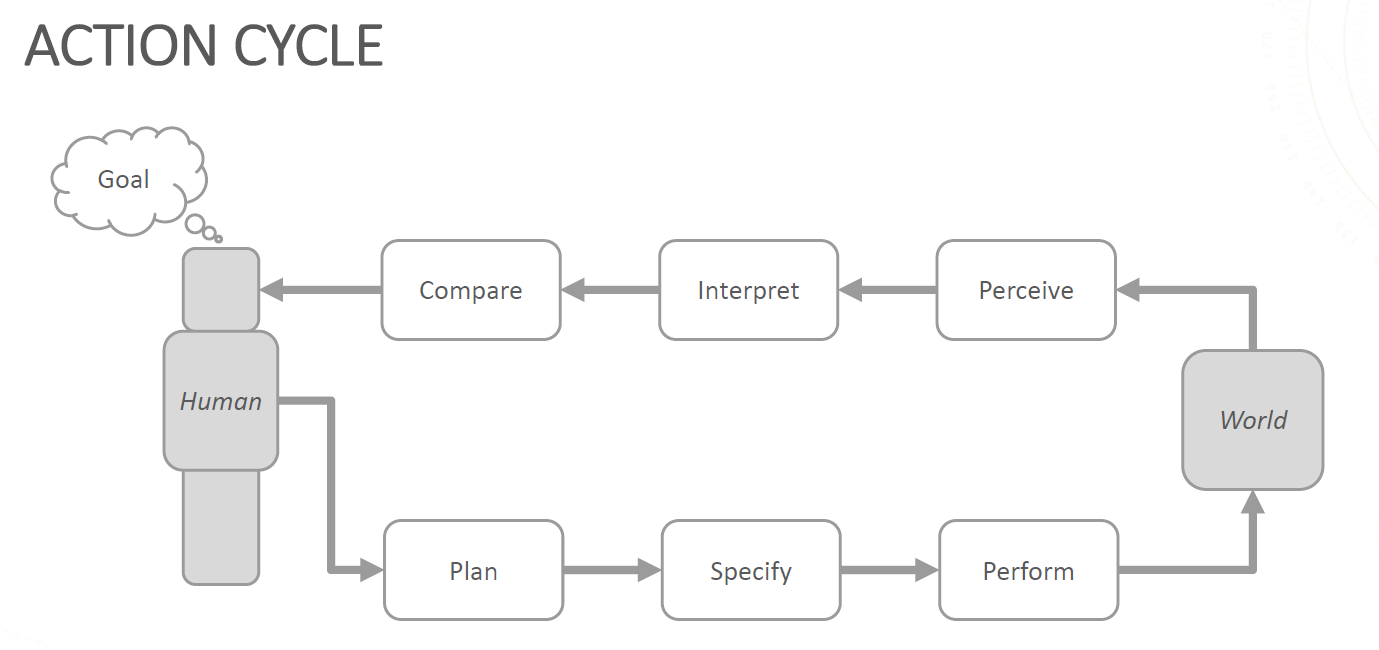
\includegraphics[scale=0.4]{img/action_cycle.png}
		\caption{Action Cylce nach Norman}
	\end{figure}
	
	\item Iteration/Bsp für den Action Cycle\\
	Am Beispiel: Kaffee holen in der Mensa
	\begin{itemize}
		\item \textbf{Goal:} Kaffee in der Mensa holen
		\item \textbf{Plan:} Aus dem Büro gehen
		\item \textbf{Specify:} Operation - Türgriff betätigen um Bürotür zu öffnen
		\item \textbf{Perform:} Türgriff drücken
		\item \textbf{Perceive:} Griff öffnet das Schloss, Tür öffnet sich
		\item \textbf{Interpret:} Tür ist offen
		\item \textbf{Compare:} Schritt erfolgreich, Führe weitere Schritte aus
	\end{itemize}
	
	
	\item  Gulf of Execution and Evalutation
	\begin{itemize}
		\item \textbf{Execution}\\
		beschreibt die Mühe/Aufwand der angestrebten Aufgaben\\
		Kann ich das tun? Wo ist die notwendige Funktionalität? Welches Gerät nutze ich? Wie führe ich das Kommando aus?
		\item \textbf{Evaluation}\\
		Beschreibt die Mühe/Aufwand die Veränderung der Umwelt zu interpretieren\\
		Ist überhaupt etwas passiert? Wo ist etwas passiert? Was ist passiert? Passen Effekt und Absicht zusammen?
		\item Interaction cost = Summe des physischen und mentalen Aufwandes um ein Ziel zu erreichen
		\item Beispielhaft am Action Cycle:
		\begin{itemize}
			\item Cost of Decision (Goal): Fokus muss auf Teilmenge von Informationen und Interfaces gelenkt werden
			\item Cost of System Power (Plan): Übersetzen von Zielen im Kopf in Operationssequenzen ist schwer, insbesondere für komplexe Systeme
			\item Cost of visual clutter/visuelle Überfuütung/reizung (Perceive): Bsp - Mouse Hover Effekte erzeugen Überreizung und erschweren Zustandswahrnehmung 
		\end{itemize}
	\end{itemize}
	
	\item The Three levels of interaction
	\begin{itemize}
		\item \textbf{low level:} Selection and Manipulation
		\item \textbf{inter-mediate level:} Exploration and Navigation
		\item \textbf{high level:} Problem-solving
	\end{itemize}
	
	\item The levels of (human) interaction processing
	\begin{itemize}
		\item Instinktiv (Perform and Perceive): vollkommen unterbewusst, ohne Kontrolle, schnell, Basisfähigkeiten - Bsp: Arm bewegen um Türgriff zu fassen
		\item Behavioral (Specify and Interpret): teilweise unterbewusst, leichte Kontrolle, schnell, gelernte Fähigkeiten - Bsp: Drücken der Klinke öffnet Tür
		\item Reflective (Plan and Compare): volles Bewusstsein, langsam, komplexe Analyse - Bsp: Tür ist offen, was bedeutet das?
	\end{itemize}
	
	\item at least 5 golden rules or guidelines for interaction\\
	\textbf{Golden Rules - Norman}
	\begin{enumerate}
		\item Discoverability: Welche (möglichen) Aktionen können bestimmt werden?
		\item Feedback: reichhaltiger und kontinuierlicher Fluss an Informationen über den Zustand
		\item Affordances: angemessene Aufforderungen um die gewünschte Aktion durchzuführen
		\item Signifiers: effiziente Signalgeber für Discoverability und Feedback
		\item Mappings: gute Zuordnung zwischen Controls and Actions
	\end{enumerate}
	\textbf{Guidelines - Shneiderman}
	\begin{enumerate}
		\item Konsistenz: ähnliche Situationen sollen ähnliche Aktionen erfordern
		\item Universal Usability: Assistenz anbieten (Hilfe, Shortcuts,..)
		\item Informative Feedback: Feedback für jede Useraktion
		\item Closure: klarer Beginn, Ablauf und Ende einer Aktion; kombiniere mit Punkt 3
		\item Prevent Error: vermeide fehlerhaften input, Recover from user error
		\item Easy reversal of actions: zb undo redo
		\item internal locus of control: User kontrolliert das System
		\item reduce short-term memory load: keep it simple
	\end{enumerate}
\end{enumerate}

\textbf{Sonstige Notizen}
\begin{itemize}
	\item Vor- und Nachteile der Interaction
	\begin{table}[!h]
		\centering
		\begin{tabular}{|p{20em}|p{20em}|}
			\hline
			\textbf{Vorteile} & \textbf{Nachteile}\\
			\hline
			\tabitem ist mächtiger als ''Algorithmen'' & \tabitem User muss wissen \textit{was} er/sie möchte\\
			\tabitem anspruchsvolleres Verhalten & \tabitem User muss wissen \textit{wie} er/sie den Computer bedienen muss um das Ziel zu erreichen\\
			 & \tabitem Anwendung ist zustandsbehaftet -> User kann sich verlieren/steckenbleiben (stateful things can be broken)\\
			\hline
		\end{tabular}
	\end{table}
	
	\item Bottlenecks - Processing: CPU, RAM, Netzwerk etc.. mittlerweile in vielen Anwendungsgebieten nicht mehr so relevant
	\item Bottlenecks - Information: enorm wichtig welche Daten auf dem kleinen Bildschirm am Ende angezeigt werden (viele, viele Daten gespeichert; welche Davon sind wichtig und werden angezeigt?)
	\item Bottlenecks - Aufnahmefähigkeit Mensch
\end{itemize}


\subsection{Basics of Graphics and Interaction Programming}
\begin{enumerate}
	\item Illustrate the interplay of the action cycle and the model-view-controller pattern!
	\begin{figure}[!h]
		\centering
		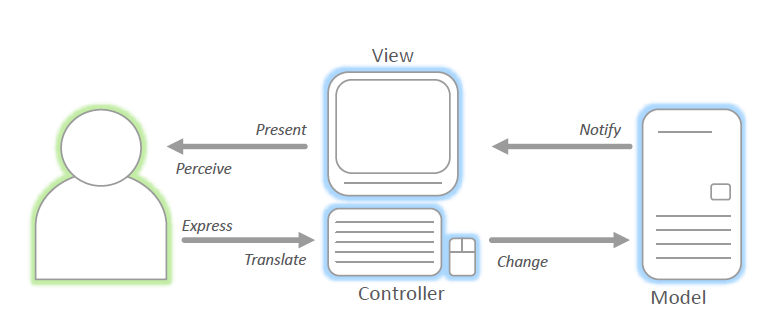
\includegraphics[scale=0.5]{img/ac_with_mvc.png}
		\caption{Zusammenspiel Action Cycle und MVC}
	\end{figure}
	
	\item Discuss different forms of presentation!\\
	Wahrnehmungen durch die 5 Sinne, geordnet nach Relevanz für HCI:\\
	Visuell, Audio, Fühlbar, Geruch, Geschmack\\
	wichtige Aspekte: Bandbreite, Aufmerksamkeit, Vergänglichkeit/Flüchtigkeit
	
	\item Discuss different forms of expression!\\
	Sprache, Point \& Gestures, Physical movement (sich selbst, Objekte wie Maus, Tastatur..)\\
	wichtige Aspekte: Genauigkeit, Geschwindigkeit, Aufwand
	
	\item Discuss pros and cons of uni-modal and multi-modal interaction!\\
	\textbf{Uni-Modal:} genau eine Form der Presentation und Expression (zb Visuell und Point \& Gestures) $\Rightarrow$ ein Kanal\\
	\textbf{Multi-Modal:} mehrere Formen/Kanäle; zb Visuell, Audio und Touch, Sprache, Point..
	\begin{table}[!h]
		\centering
		\begin{tabular}{|l|p{15em}|p{15em}|}
			\hline
			&	\textbf{Vorteile} & \textbf{Nachteile}\\
			\hline
			Uni-Modal & einfache Implementierung & nur ein Kanal\\
			\hline
			Multi-Modal & umfangreiche Formen der Interaktion & komplexe Implementierung und schwieriger zu lernen (für den User)\\
			\hline
		\end{tabular}
	\end{table}
	
	\item What are the mental, implementation and represented model? Why are they important?
	\begin{itemize}
		\item \textbf{Mental:} gedankliche Vorstellung des Modells; entspricht menschlicher Natur; beschreibt v.a. Operationen zum Erreichen des Ziels
		\item \textbf{Implementation:} interne Darstellung; technisch limitiert und vom Entwickler vorgegeben; enthält Daten, Parameter, Algorithmen,...
		\item \textbf{Represented:} Darstellung des (Implementation) Models auf dem PC; vom Entwickler vorgegeben;
	\end{itemize}
	
	\begin{figure}[!h]
		\centering
		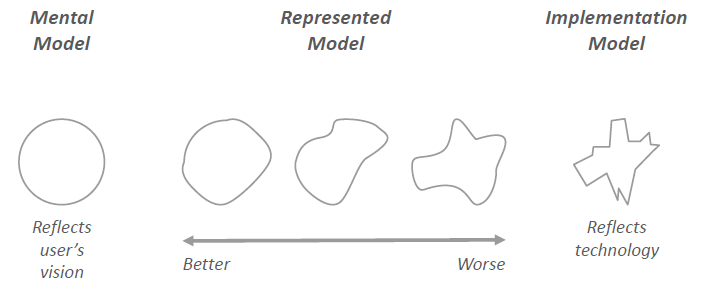
\includegraphics[scale=0.5]{img/models.png}
		\caption{Zusammenspiel der 3 Modelle}
	\end{figure}
	\textit{Important}, weil Mental Model nicht 1:1 in Computer dargestellt werden kann; müssen abstrahieren
	
	\item What is a graphics context and what can it be used for?\\
	Wird gestellt vom Window System und ist verknüpft mit dem Zeichenareal.\\
	Stellt Funktionalitäten zum Zeichnen bereit.
	
	\item Explain the basic procedure for drawing paths!\\
	begin path; move to; add (line, curve, arc,..); end path
	
	\item Name three interaction devices and characterize the input they deliver\\
	Pointing Device (Maus): absolute oder relative Koordinaten\\
	Triggers (Tasten)\\
	Value Input (Sensoren)

	\item Give examples of atomic and composite inputs!\\
	atomic: single click, Bewegung des Zeigers, aktiviere Trigger,..\\
	composite: double click, drag n drop, Gesten,...
	
	\item Illustrate the interconnections between model, view and controller in MVC pattern!
	\begin{figure}[!h]
		\centering
		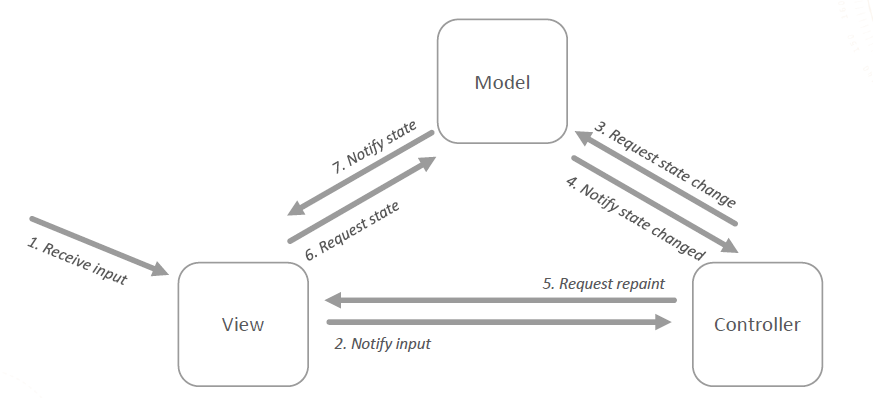
\includegraphics[scale=0.5]{img/mvc_interconnection.png}
		\caption{Interconnection der drei Bestandteile des MVC Pattern}
	\end{figure}
	
	\item Discuss advantages and disadvantes of the MVC!
	\begin{table}[!h]
		\centering
		\begin{tabular}{|p{20em}|p{20em}|}
			\hline
			\textbf{Vorteile} & \textbf{Nachteile}\\
			\hline
			klare konzeptuelle Trennung der Bestandteile & \tabitem enge Kopplung der Komponenten (durch Interaktion)\\
			\tabitem Entwurf für generelle Architektur & \tabitem komplex zu implementieren\\
			\hline
		\end{tabular}
	\end{table}
	
	\item What loop is the fundamental ingredient of interactive systems!\\
	\textbf{event loop:} Endlosschleife von Reaktionen auf Events; verschiedene Eventtypen; verschiedene Reaktionen
	
	\item Name at least five types of events in interaction systems!
	\begin{itemize}
		\item Application level: loaded, finished,..
		\item Widget level: Repaint, Resize, Activated, focused,...
		\item Input level: key pressed/released/typed,.. Touch start/moved/end, Mouse pressed/...
		\item Window System signals external event: repaint of window required; resize of window; Input von Peripherie (zb Maus)
		\item Application signals internal events: state change, timer elapsed
	\end{itemize}
	
	\item How are events propagated in interactive systems?\\
	Werden in EventQueue reingesteckte und nach FIFO verarbeitet;\\
	Dispatch Events: Traversiere Window Tree und wähle vorderstes Fensters aus\\
	Receive Events: definiere Verhalten bei Event; ausgeführt durch Listener
	
	\item How can callback functions be used to react to events?\\
	Callback als Parameter einer Funktion -> Funktion ausgeführt, dann führe Callback aus. Auf Events: Ich sage Programm mach etwas und du sollst mir Bescheid geben(=callback), Ausführung erzeugt Event und callback wird gerufen(omfg.. xD)\\
	gut für basic (device) events; but limited flexibility
	
	\item What are delegates and listeners?
	Interface um auf Events zu reagieren; Logik muss vom Entwickler umgesetzt werden\\
	cover many different events, also user-generated ones; but sometimes clomplex
	
	\item What are signals and slots and which toolkits make use of them?
	QT, GTK+,.. Kommunikation zwischen Objekten; Signal wird emitted wenn Event auftritt; Slot = Funktion die bei bestimmtem Event aufgerufen wird\\
	ähnlich zu Callbacks, aber mit höherer Flexibilität
	
	\item Express in pseudo code the main event loop and explain its components!\\
	Block and render -> wartet auf Event und rendert nur bei Bedarf neu
	\begin{lstlisting}
	while (true || event != QUIT) {
		event = wait_for_event();
		do_repaint = update_model(event)
		if (do_repaint) {
			render_model()
		}
	}
	\end{lstlisting}
	check and render full-throttle -> render mit jedem Durchlauf und reagiert nur auf Events
	\begin{lstlisting}
	while (true || event != QUIT) {
		if (check_for_event()) {
			event = get_event()
			update_model(event)
		}
		render_model()
	}
	\end{lstlisting}
		
	\item What is a disadvantage of method overriding for reacting to events?
	sollte in Sub-Class ausgelagert werden um Custom Verhalten umzusetzen; im Gegensatz zum Listener Konzept wesentlich unübersichtlicherer Code
	
\end{enumerate}